%!TeX root=../pridetop.tex
\chapter[Chapter \thechapter]{}
	
	
\begin{figure}[t!]
\centering

\includegraphics[width=\linewidth]{61top}
\captionlistentry{Headpiece to Chapter \thechapter}
\end{figure}


\lettrine[lines=6,image=true]{initials/chap61h}{appy} for all her maternal feelings was the day on which Mrs Bennet got rid of her two most deserving daughters. With what delighted pride she afterwards visited Mrs Bingley, and talked of Mrs Darcy, may be guessed. I wish I could say, for the sake of her family, that the accomplishment of her earnest desire in the establishment of so many of her children produced so happy an effect as to make her a sensible, amiable, well-informed woman for the rest of her life; though, perhaps, it was lucky for her husband, who might not have relished domestic felicity in so unusual a form, that she still was occasionally nervous and invariably silly.

Mr Bennet missed his second daughter exceedingly; his affection for her drew him oftener from home than anything else could do. He delighted in going to Pemberley, especially when he was least expected.

Mr Bingley and Jane remained at Netherfield only a twelvemonth. So near a vicinity to her mother and Meryton relations was not desirable even to \textit{his} easy temper, or \textit{her} affectionate heart. The darling wish of his sisters was then gratified: he bought an estate in a neighbouring county to Derbyshire; and Jane and Elizabeth, in addition to every other source of happiness, were within thirty miles of each other.

Kitty, to her very material advantage, spent the chief of her time with her two elder sisters. In society so superior to what she had generally known, her improvement was great. She was not of so ungovernable a temper as Lydia; and, removed from the influence of Lydia's example, she became, by proper attention and management, less irritable, less ignorant, and less insipid. From the further disadvantage of Lydia's society she was of course carefully kept; and though Mrs Wickham frequently invited her to come and stay with her, with the promise of balls and young men, her father would never consent to her going.

Mary was the only daughter who remained at home; and she was necessarily drawn from the pursuit of accomplishments by Mrs Bennet's being quite unable to sit alone. Mary was obliged to mix more with the world, but she could still moralize over every morning visit; and as she was no longer mortified by comparisons between her sisters' beauty and her own, it was suspected by her father that she submitted to the change without much reluctance.

As for Wickham and Lydia, their characters suffered no revolution from the marriage of her sisters. He bore with philosophy the conviction that Elizabeth must now become acquainted with whatever of his ingratitude and falsehood had before been unknown to her; and, in spite of everything, was not wholly without hope that Darcy might yet be prevailed on to make his fortune. The congratulatory letter which Elizabeth received from Lydia on her marriage explained to her that, by his wife at least, if not by himself, such a hope was cherished. The letter was to this effect:—

\begin{mail}{}{My dear Lizzy,}

I wish you joy. If you love Mr Darcy half so well as I do my dear Wickham, you must be very happy. It is a great comfort to have you so rich; and when you have nothing else to do, I hope you will think of us. I am sure Wickham would like a place at court very much; and I do not think we shall have quite money enough to live upon without some help. Any place would do of about three or four hundred a year; but, however, do not speak to Mr Darcy about it, if you had rather not.
\closeletter[Yours, etc.]{}
\end{mail}

As it happened that Elizabeth had much rather not, she endeavoured in her answer to put an end to every entreaty and expectation of the kind. Such relief, however, as it was in her power to afford, by the practice of what might be called economy in her own private expenses, she frequently sent them. It had always been evident to her that such an income as theirs, under the direction of two persons so extravagant in their wants, and heedless of the future, must be very insufficient to their support; and whenever they changed their quarters, either Jane or herself were sure of being applied to for some little assistance towards discharging their bills. Their manner of living, even when the restoration of peace dismissed them to a home, was unsettled in the extreme. They were always moving from place to place in quest of a cheap situation, and always spending more than they ought. His affection for her soon sunk into indifference: hers lasted a little longer; and, in spite of her youth and her manners, she retained all the claims to reputation which her marriage had given her. Though Darcy could never receive \textit{him} at Pemberley, yet, for Elizabeth's sake, he assisted him further in his profession. Lydia was occasionally a visitor there, when her husband was gone to enjoy himself in London or Bath; and with the Bingleys they both of them frequently stayed so long, that even Bingley's good-humour was overcome, and he proceeded so far as to \textit{talk} of giving them a hint to be gone.

Miss Bingley was very deeply mortified by Darcy's marriage; but as she thought it advisable to retain the right of visiting at Pemberley, she dropped all her resentment; was fonder than ever of Georgiana, almost as attentive to Darcy as heretofore, and paid off every arrear of civility to Elizabeth.

Pemberley was now Georgiana's home; and the attachment of the sisters was exactly what Darcy had hoped to see. They were able to love each other, even as well as they intended. Georgiana had the highest opinion in the world of Elizabeth; though at first she often listened with an astonishment bordering on alarm at her lively, sportive manner of talking to her brother. He, who had always inspired in herself a respect which almost overcame her affection, she now saw the object of open pleasantry. Her mind received knowledge which had never before fallen in her way. By Elizabeth's instructions she began to comprehend that a woman may take liberties with her husband, which a brother will not always allow in a sister more than ten years younger than himself.

Lady Catherine was extremely indignant on the marriage of her nephew; and as she gave way to all the genuine frankness of her character, in her reply to the letter which announced its arrangement, she sent him language so very abusive, especially of Elizabeth, that for some time all intercourse was at an end. But at length, by Elizabeth's persuasion, he was prevailed on to overlook the offence, and seek a reconciliation; and, after a little further resistance on the part of his aunt, her resentment gave way, either to her affection for him, or her curiosity to see how his wife conducted herself; and she condescended to wait on them at Pemberley, in spite of that pollution which its woods had received, not merely from the presence of such a mistress, but the visits of her uncle and aunt from the city.

With the Gardiners they were always on the most intimate terms. Darcy, as well as Elizabeth, really loved them; and they were both ever sensible of the warmest gratitude towards the persons who, by bringing her into Derbyshire, had been the means of uniting them.

%\begin{figure}[b!]
%\centering
%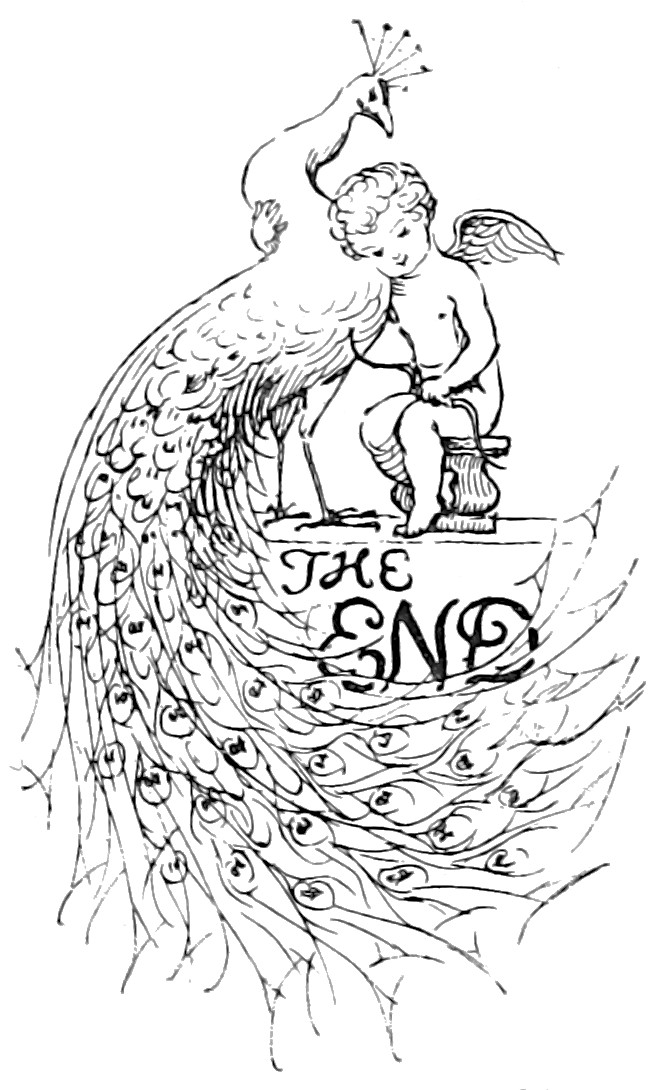
\includegraphics[width=.5\linewidth]{theend}
%\captionlistentry{The End}
%\end{figure}

\begin{a4}
	\begin{tikzpicture}[remember picture, overlay]  
		\node (theend) at ($(current page.south)+(0cm,4cm)$) {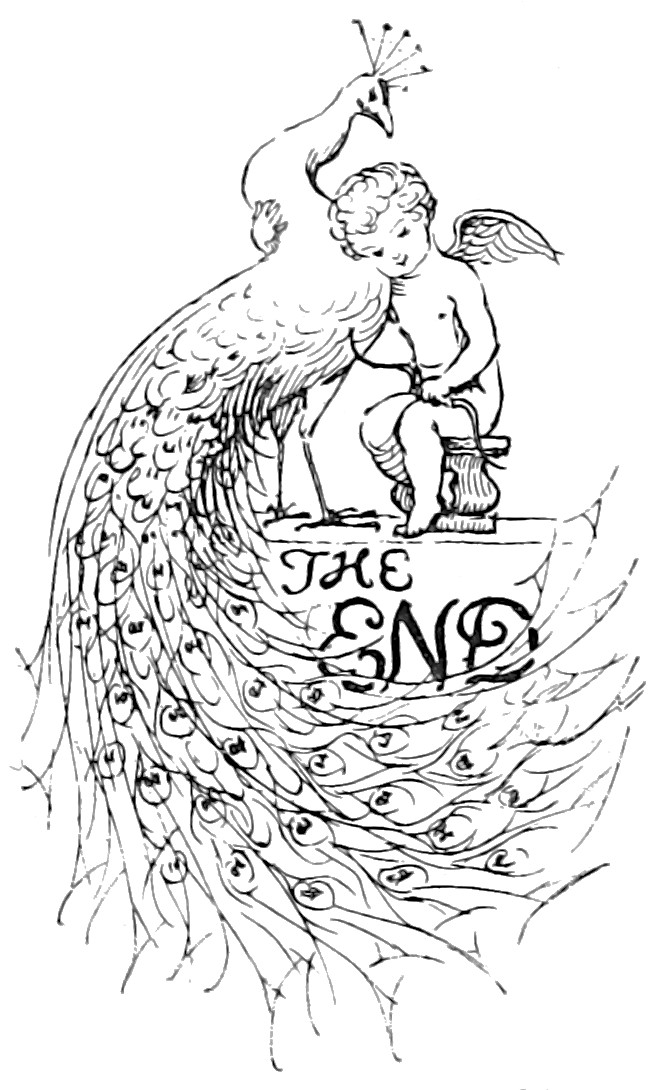
\includegraphics[width=.35\linewidth]{theend}};
	\end{tikzpicture}
	\captionof{figure}[The End]{}
\end{a4}

\begin{letter}
	\begin{tikzpicture}[remember picture, overlay]  
		\node (theend) at ($(current page.south)+(0cm,5cm)$) {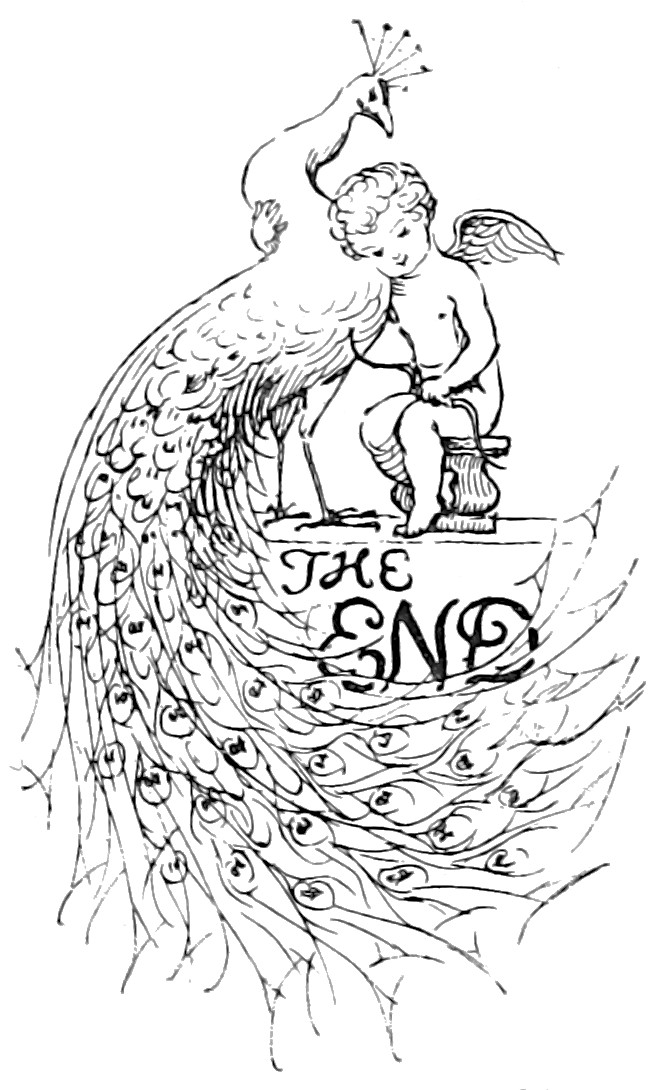
\includegraphics[width=.45\linewidth]{theend}};
	\end{tikzpicture}
	\captionof{figure}[The End]{}
\end{letter}